%==============================================================================
%  Exercise 3 --- Thống kê nhiều chiều & cao chiều (Johnson--Wichern, Chương 4--5)
%  Theo templates/hmmt-solution-template.tex (phong cách Harvard-MIT Math Tournament)
%  - Chỉ trắng và đen: không màu, không khung, không tcolorbox, không đổ bóng.
%  - Tiêu đề gọn ở giữa trang, không trang bìa, không \maketitle.
%  - Đề bài chạy dòng ("1." / "Bài 2.1." in đậm), lời giải run-in "Lời giải:".
%  - Đáp số cuối cùng đóng khung bằng \boxed{...}.
%  Biên dịch: xelatex (bắt buộc, vì dùng fontspec + polyglossia + unicode-math)
%==============================================================================
\documentclass[11pt,a4paper]{article}

% --- Ngôn ngữ và font: Latin Modern (Computer Modern) như bản HMMT gốc -------
\usepackage{fontspec}
\usepackage{polyglossia}
\setdefaultlanguage{vietnamese}
\setmainfont{lmroman10-regular.otf}[
  BoldFont       = lmroman10-bold.otf,
  ItalicFont     = lmroman10-italic.otf,
  BoldItalicFont = lmroman10-bolditalic.otf
]

% --- Toán học ---------------------------------------------------------------
\usepackage{amsmath, amssymb, amsthm}
\usepackage{unicode-math}
\setmathfont{latinmodern-math.otf}
\renewcommand{\boldsymbol}[1]{\symbf{#1}}
\allowdisplaybreaks

% --- Khổ trang: lề rộng, khối chữ gọn vào giữa ------------------------------
\usepackage[a4paper, top=2.5cm, bottom=2.5cm, left=2.7cm, right=2.7cm]{geometry}
\usepackage{enumitem}
\usepackage{graphicx}
\usepackage{booktabs}
\usepackage[hidelinks]{hyperref}
\setlist{itemsep=5pt, topsep=6pt, parsep=2pt, partopsep=0pt, leftmargin=1.8em}

% Đoạn văn kiểu HMMT: thụt đầu dòng, KHÔNG dùng parskip (không chèn dòng trống)
\setlength{\parindent}{1.5em}
\setlength{\parskip}{0pt}
\setlength{\abovedisplayskip}{5pt plus 1pt minus 2pt}
\setlength{\belowdisplayskip}{5pt plus 1pt minus 2pt}
\setlength{\abovedisplayshortskip}{2pt plus 1pt}
\setlength{\belowdisplayshortskip}{2pt plus 1pt}

% Chỉ số trang canh giữa chân trang, không running header
\pagestyle{plain}
\raggedbottom

% --- Thông tin tài liệu (sửa 4 dòng này cho mỗi bài) ------------------------
\newcommand{\coursename}{Thống kê nhiều chiều}
\newcommand{\docdate}{\today}
\newcommand{\doctitle}{Lời giải bài tập về nhà -- Exercise 3}
\newcommand{\studentname}{Quang Nguyễn}

% --- Đề bài / lời giải ------------------------------------------------------
\newcounter{prob}
\makeatletter
% \begin{problem}            -> tự đánh số 1., 2., 3., ...
% \begin{problem}[Bài 2.1.]  -> dùng nhãn tự đặt
\newenvironment{problem}[1][]{%
  \par\addvspace{14pt}\noindent\begin{minipage}{\linewidth}
  \def\@tempa{#1}%
  \ifx\@tempa\@empty\refstepcounter{prob}\textbf{\theprob.}\else\textbf{#1}\fi
  \ \ignorespaces
}{\par\end{minipage}\par\nopagebreak[4]}
\makeatother

% Lời giải: tiêu đề riêng dòng, tách rõ khỏi các ý của đề bài.
\newenvironment{solution}{%
  \par\medskip\noindent\textbf{Lời giải:}\par\nobreak\smallskip\noindent\ignorespaces
}{\par}

% Đáp số cuối cùng luôn đóng khung
\newcommand{\answer}[1]{\boxed{#1}}

\begin{document}

%------------------------------ Tiêu đề gọn ---------------------------------
\begin{center}
  {\bfseries\coursename}\\
  \docdate\\
  \doctitle: \textbf{\studentname}
\end{center}
\vspace{0.5em}


\noindent\textit{Phạm vi.} Lời giải cho 22 bài được chỉ định trong Johnson--Wichern,
\textit{Applied Multivariate Statistical Analysis}, ấn bản 6, Chương 4--5.
Các nhãn bài theo sách; phần đề chỉ ghi tóm tắt, các phép tính và chứng minh
được trình bày độc lập. Dữ kiện được đối chiếu với bản sách, không suy ra
chỉ từ sự tương đồng với Exercise 1--2.

\medskip
\noindent\textbf{Quy ước và công thức dùng chung.}
Với mẫu $\mathbf{x}_1,\ldots,\mathbf{x}_n\in\mathbb R^p$, đặt
\[
\bar{\mathbf{x}}=\frac1n\sum_i\mathbf{x}_i,\qquad
\mathbf S=\frac1{n-1}\sum_i(\mathbf{x}_i-\bar{\mathbf{x}})
(\mathbf{x}_i-\bar{\mathbf{x}})'.
\]
Các phân vị $F_{a,b}(q)$, $t_\nu(q)$ và $\chi_p^2(q)$ là phân vị tích lũy mức $q$.
Với mẫu chuẩn, $\boldsymbol\Sigma>0$ và $n>p$, dưới $H_0:\boldsymbol\mu=\boldsymbol\mu_0$,
\[
T^2=n(\bar{\mathbf x}-\boldsymbol\mu_0)'\mathbf S^{-1}
(\bar{\mathbf x}-\boldsymbol\mu_0),\qquad
\frac{n-p}{p(n-1)}T^2\sim F_{p,n-p}.
\]
Đặt $c_T=\frac{p(n-1)}{n-p}F_{p,n-p}(1-\alpha)$. Miền tin cậy là
$n(\bar{\mathbf x}-\boldsymbol\mu)'\mathbf S^{-1}(\bar{\mathbf x}-\boldsymbol\mu)\le c_T$.
Khoảng đồng thời cho mọi tổ hợp tuyến tính là
\[
\mathbf a'\bar{\mathbf x}\pm\sqrt{c_T\mathbf a'\mathbf S\mathbf a/n}.
\]
Với $m$ đại lượng được chỉ định trước, Bonferroni dùng
$t_{n-1}(1-\alpha/(2m))$ thay cho $\sqrt{c_T}$.
Khi chỉ có giả thiết mẫu lớn và số chiều cố định, dùng $\chi_p^2(1-\alpha)$
thay cho $c_T$; tính chính xác của phân phối $F$ đòi hỏi mẫu chuẩn.

\begin{center}\textbf{Chương 4. Phân phối chuẩn nhiều chiều}\end{center}

\begin{problem}[Bài 4.3.]
Tính độc lập của các thành phần và tổ hợp tuyến tính.
\end{problem}
\begin{solution}
Dữ kiện là $\boldsymbol\mu=(-3,1,4)'$ và
\[
\boldsymbol\Sigma=\begin{pmatrix}1&-2&0\\-2&5&0\\0&0&2\end{pmatrix}.
\]
Mọi vectơ ghép từ các tổ hợp tuyến tính của $\mathbf X$ đều chuẩn đồng thời.
Do đó độc lập tương đương với ma trận hiệp phương sai chéo bằng không.
\begin{enumerate}[label=\textbf{\alph*)}]
\item $\operatorname{Cov}(X_1,X_2)=-2\ne0$: \textbf{không độc lập}.
\item $\operatorname{Cov}(X_2,X_3)=0$: \textbf{độc lập}.
\item $\operatorname{Cov}((X_1,X_2)',X_3)=(0,0)'$: \textbf{độc lập}.
\item $\operatorname{Cov}((X_1+X_2)/2,X_3)=(0+0)/2=0$: \textbf{độc lập}.
\item Đặt $W=X_2-\frac52X_1-X_3$. Khi đó
\[
\operatorname{Cov}(X_2,W)=5-\frac52(-2)-0=10\ne0,
\]
 nên $X_2$ và $W$ \textbf{không độc lập}.
\end{enumerate}
\[
\answer{\text{Độc lập: (b), (c), (d); không độc lập: (a), (e).}}
\]
Lưu ý dấu trừ ở câu (e): hệ số $-5/2$ không triệt tiêu hiệp phương sai.
\end{solution}

\begin{problem}[Bài 4.4.]
Phân phối của tổ hợp tuyến tính và lựa chọn hệ số để có tính độc lập.
\end{problem}
\begin{solution}
Ở đây
\[
\boldsymbol\mu=(2,-3,1)',\qquad
\boldsymbol\Sigma=\begin{pmatrix}1&1&1\\1&3&2\\1&2&2\end{pmatrix}.
\]
\begin{enumerate}[label=\textbf{\alph*)}]
\item Với $\mathbf c=(3,-2,1)'$, $Y=\mathbf c'\mathbf X$ là biến chuẩn.
Ta có
\[
E(Y)=3(2)-2(-3)+1=13,\qquad
\boldsymbol\Sigma\mathbf c=(2,-1,1)',
\]
\[
\operatorname{Var}(Y)=\mathbf c'\boldsymbol\Sigma\mathbf c
=3(2)+(-2)(-1)+1=9.
\]
Vậy $\answer{3X_1-2X_2+X_3\sim\mathcal N(13,9)}$.
\item Đặt $W=X_2-a_1X_1-a_2X_3$. Cặp $(X_2,W)$ chuẩn đồng thời và
\[
\operatorname{Cov}(X_2,W)=3-a_1-2a_2.
\]
Vì vậy toàn bộ nghiệm là
\[
\answer{\mathbf a=(3-2t,t)',\quad t\in\mathbb R.}
\]
Chẳng hạn, $\mathbf a=(1,1)'$ cho $X_2$ độc lập với $X_2-X_1-X_3$.
Điều kiện đề yêu cầu là độc lập với $X_2$; không được thay bằng điều kiện
phần dư độc lập với vectơ $(X_1,X_3)'$, vốn là một bài toán khác.
\end{enumerate}
\end{solution}

\begin{problem}[Bài 4.5.]
Ba phân phối có điều kiện, dùng dữ kiện của Bài 4.2, 4.3 và 4.4.
\end{problem}
\begin{solution}
Công thức dùng chung cho vectơ chuẩn phân hoạch $(\mathbf U',\mathbf V')'$ là
\[
\mathbf U\mid\mathbf V=\mathbf v\sim\mathcal N\bigl(
\boldsymbol\mu_U+\boldsymbol\Sigma_{UV}\boldsymbol\Sigma_{VV}^{-1}
(\mathbf v-\boldsymbol\mu_V),\;
\boldsymbol\Sigma_{UU}-\boldsymbol\Sigma_{UV}\boldsymbol\Sigma_{VV}^{-1}
\boldsymbol\Sigma_{VU}\bigr).
\]
\begin{enumerate}[label=\textbf{\alph*)}]
\item Bài 4.2 cho $\mu_1=0,\mu_2=2,\sigma_{11}=2,\sigma_{22}=1,\rho_{12}=1/2$.
Do đó $\sigma_{12}=\rho_{12}\sqrt{\sigma_{11}\sigma_{22}}=1/\sqrt2$ và
\[
E(X_1\mid X_2=x_2)=\frac{x_2-2}{\sqrt2},\qquad
\operatorname{Var}(X_1\mid X_2)=2-\frac12=\frac32.
\]
Suy ra
\[
\answer{X_1\mid X_2=x_2\sim\mathcal N\left(\frac{x_2-2}{\sqrt2},\frac32\right).}
\]
\item Trong Bài 4.3, $\mathbf V=(X_1,X_3)'$ có kỳ vọng $(-3,4)'$,
$\boldsymbol\Sigma_{VV}=\operatorname{diag}(1,2)$ và
$\boldsymbol\Sigma_{2V}=(-2,0)$. Vậy
\[
E(X_2\mid\mathbf V)=1-2(x_1+3)=-2x_1-5,\qquad
\operatorname{Var}(X_2\mid\mathbf V)=5-4=1.
\]
\[
\answer{X_2\mid(X_1=x_1,X_3=x_3)\sim\mathcal N(-2x_1-5,1).}
\]
\item Trong Bài 4.4, đặt $\mathbf V=(X_1,X_2)'$. Khi đó
\[
\boldsymbol\Sigma_{VV}=\begin{pmatrix}1&1\\1&3\end{pmatrix},\quad
\boldsymbol\Sigma_{VV}^{-1}=\frac12\begin{pmatrix}3&-1\\-1&1\end{pmatrix},\quad
\boldsymbol\Sigma_{3V}=(1,2).
\]
Hệ số hồi quy là $(1,2)\boldsymbol\Sigma_{VV}^{-1}=(1/2,1/2)$, nên
\[
E(X_3\mid\mathbf V)=1+\tfrac12(x_1-2)+\tfrac12(x_2+3)
=\tfrac32+\tfrac12(x_1+x_2),
\]
\[
\operatorname{Var}(X_3\mid\mathbf V)=2-(1/2,1/2)(1,2)'=\tfrac12.
\]
\[
\answer{X_3\mid(X_1=x_1,X_2=x_2)\sim
\mathcal N\left(\frac{3+x_1+x_2}{2},\frac12\right).}
\]
\end{enumerate}
\end{solution}

\begin{problem}[Bài 4.6.]
Kiểm tra năm quan hệ độc lập.
\end{problem}
\begin{solution}
Dữ kiện $\boldsymbol\mu=(1,-1,2)'$ và
\[
\boldsymbol\Sigma=\begin{pmatrix}4&0&-1\\0&5&0\\-1&0&2\end{pmatrix}.
\]
Dùng tính chuẩn đồng thời, ta có
\begin{enumerate}[label=\textbf{\alph*)}]
\item $\operatorname{Cov}(X_1,X_2)=0$: độc lập.
\item $\operatorname{Cov}(X_1,X_3)=-1$: không độc lập.
\item $\operatorname{Cov}(X_2,X_3)=0$: độc lập.
\item $\operatorname{Cov}((X_1,X_3)',X_2)=(0,0)'$: độc lập.
\item $\operatorname{Cov}(X_1,X_1+3X_2-2X_3)=4+3(0)-2(-1)=6$: không độc lập.
\end{enumerate}
\[
\answer{\text{Độc lập: (a), (c), (d); không độc lập: (b), (e).}}
\]
\end{solution}

\begin{problem}[Bài 4.7.]
Phân phối có điều kiện từ dữ kiện Bài 4.6.
\end{problem}
\begin{solution}
\begin{enumerate}[label=\textbf{\alph*)}]
\item Ta có
\[
E(X_1\mid X_3=x_3)=1+\frac{-1}{2}(x_3-2)=2-\frac{x_3}{2},\qquad
\operatorname{Var}(X_1\mid X_3)=4-\frac{(-1)^2}{2}=\frac72.
\]
Vậy
\[
\answer{X_1\mid X_3=x_3\sim\mathcal N(2-x_3/2,7/2).}
\]
\item Vì $X_2$ độc lập với cả vectơ $(X_1,X_3)'$, việc biết thêm $X_2=x_2$
không thay đổi phân phối trên. Có thể kiểm tra trực tiếp:
\[
(0,-1)\begin{pmatrix}5&0\\0&2\end{pmatrix}^{-1}=(0,-1/2).
\]
Do đó
\[
\answer{X_1\mid(X_2=x_2,X_3=x_3)\sim\mathcal N(2-x_3/2,7/2).}
\]
\end{enumerate}
\end{solution}

\begin{problem}[Bài 4.16.]
Phân phối biên và mật độ đồng thời của hai tổ hợp vectơ chuẩn độc lập.
\end{problem}
\begin{solution}
Bốn vectơ $\mathbf X_j$ độc lập, cùng phân phối $\mathcal N_p(\boldsymbol\mu,\boldsymbol\Sigma)$.
Các hệ số trong sách đều có mẫu số $4$:
\[
\mathbf V_1=\frac{\mathbf X_1-\mathbf X_2+\mathbf X_3-\mathbf X_4}{4},\qquad
\mathbf V_2=\frac{\mathbf X_1+\mathbf X_2-\mathbf X_3-\mathbf X_4}{4}.
\]
\begin{enumerate}[label=\textbf{\alph*)}]
\item Tổng hệ số của mỗi tổ hợp bằng $0$, tổng bình phương hệ số bằng $4/16=1/4$.
Bởi tính độc lập giữa các quan sát,
\[
E(\mathbf V_k)=\mathbf0,\qquad\operatorname{Cov}(\mathbf V_k)=\frac14\boldsymbol\Sigma.
\]
Do tổ hợp tuyến tính của các vectơ chuẩn độc lập vẫn chuẩn,
\[
\answer{\mathbf V_1,\mathbf V_2\sim\mathcal N_p(\mathbf0,\boldsymbol\Sigma/4).}
\]
\item Hiệp phương sai chéo là
\[
\operatorname{Cov}(\mathbf V_1,\mathbf V_2)
=\frac{1-1-1+1}{16}\boldsymbol\Sigma=\mathbf0.
\]
Vectơ ghép chuẩn đồng thời nên $\mathbf V_1\perp\!\!\!\perp\mathbf V_2$ và
\[
\begin{pmatrix}\mathbf V_1\\\mathbf V_2\end{pmatrix}
\sim\mathcal N_{2p}\left(\mathbf0,
\begin{pmatrix}\boldsymbol\Sigma/4&0\\0&\boldsymbol\Sigma/4\end{pmatrix}\right).
\]
Nếu $\boldsymbol\Sigma>0$, nhân hai mật độ biên thu được
\[
\answer{f(\mathbf v_1,\mathbf v_2)=\frac{4^p}{(2\pi)^p|\boldsymbol\Sigma|}
\exp\{-2(\mathbf v_1'\boldsymbol\Sigma^{-1}\mathbf v_1+
\mathbf v_2'\boldsymbol\Sigma^{-1}\mathbf v_2)\}.}
\]
\end{enumerate}
\end{solution}

\begin{problem}[Bài 4.17.]
Kỳ vọng và hiệp phương sai của hai tổ hợp từ năm vectơ i.i.d.
\end{problem}
\begin{solution}
Đặt $\mathbf U=(\mathbf X_1+\cdots+\mathbf X_5)/5$ và
$\mathbf V=\mathbf X_1-\mathbf X_2+\mathbf X_3-\mathbf X_4+\mathbf X_5$.
Không cần giả thiết chuẩn để tính các moment. Theo tính tuyến tính,
\[
E(\mathbf U)=\frac55\boldsymbol\mu=\boldsymbol\mu,\qquad
E(\mathbf V)=(1-1+1-1+1)\boldsymbol\mu=\boldsymbol\mu.
\]
Các hiệp phương sai giữa quan sát khác nhau bằng không, vì vậy
\[
\answer{\operatorname{Cov}(\mathbf U)=\frac15\boldsymbol\Sigma,\qquad
\operatorname{Cov}(\mathbf V)=5\boldsymbol\Sigma.}
\]
Ngoài ra,
\[
\answer{\operatorname{Cov}(\mathbf U,\mathbf V)
=\frac{1-1+1-1+1}{5}\boldsymbol\Sigma=\frac15\boldsymbol\Sigma.}
\]
Nếu $\boldsymbol\Sigma\ne0$, hai vectơ không độc lập. Đề này không giả thiết
chuẩn, nên không thể tự kết luận các tổ hợp có phân phối chuẩn chính xác.
\end{solution}

\begin{problem}[Bài 4.19.]
Các phân phối mẫu khi $n=20$, $p=6$ và tổng thể chuẩn.
\end{problem}
\begin{solution}
\begin{enumerate}[label=\textbf{\alph*)}]
\item Đặt $\mathbf Z=\boldsymbol\Sigma^{-1/2}(\mathbf X_1-\boldsymbol\mu)$.
Khi đó $\mathbf Z\sim\mathcal N_6(0,I)$, nên
\[
\answer{(\mathbf X_1-\boldsymbol\mu)'\boldsymbol\Sigma^{-1}
(\mathbf X_1-\boldsymbol\mu)=\sum_{j=1}^6Z_j^2\sim\chi_6^2.}
\]
\item Trung bình của các vectơ chuẩn độc lập vẫn chuẩn, với hiệp phương sai
$20\boldsymbol\Sigma/20^2=\boldsymbol\Sigma/20$. Vì vậy
\[
\answer{\bar{\mathbf X}\sim\mathcal N_6(\boldsymbol\mu,\boldsymbol\Sigma/20),
\qquad\sqrt{20}(\bar{\mathbf X}-\boldsymbol\mu)\sim\mathcal N_6(0,\boldsymbol\Sigma).}
\]
\item Định lý phân phối mẫu chuẩn cho
\[
\answer{19\mathbf S\sim W_6(19,\boldsymbol\Sigma).}
\]
Quy ước $W_p(\nu,\boldsymbol\Sigma)$ là phân phối của
$\sum_{i=1}^{\nu}\mathbf Z_i\mathbf Z_i'$ với $\mathbf Z_i$ độc lập,
$\mathcal N_p(0,\boldsymbol\Sigma)$; vì thế $E(19\mathbf S)=19\boldsymbol\Sigma$.
Ngoài ra, $\bar{\mathbf X}$ độc lập với $\mathbf S$.
\end{enumerate}
\end{solution}

\begin{problem}[Bài 4.20.]
Biến đổi ma trận Wishart trong Bài 4.19.
\end{problem}
\begin{solution}
Viết $19\mathbf S\stackrel d=\sum_{i=1}^{19}\mathbf Z_i\mathbf Z_i'$,
$\mathbf Z_i\sim\mathcal N_6(0,\boldsymbol\Sigma)$ độc lập. Khi đó
\[
\mathbf B(19\mathbf S)\mathbf B'=\sum_{i=1}^{19}
(\mathbf B\mathbf Z_i)(\mathbf B\mathbf Z_i)',\qquad
\mathbf B\mathbf Z_i\sim\mathcal N_2(0,\mathbf B\boldsymbol\Sigma\mathbf B').
\]
Cả hai ma trận $\mathbf B$ dưới đây có hạng hàng bằng $2$, nên
\[
\answer{\mathbf B(19\mathbf S)\mathbf B'\sim W_2(19,\mathbf B\boldsymbol\Sigma\mathbf B').}
\]
\begin{enumerate}[label=\textbf{\alph*)}]
\item Với
$\mathbf B=\begin{pmatrix}1&-1/2&-1/2&0&0&0\\0&0&0&-1/2&-1/2&1\end{pmatrix}$,
viết ma trận tham số là $\begin{pmatrix}q_{11}&q_{12}\\q_{12}&q_{22}\end{pmatrix}$, trong đó
\begin{align*}
q_{11}&=\sigma_{11}+\tfrac14\sigma_{22}+\tfrac14\sigma_{33}
-\sigma_{12}-\sigma_{13}+\tfrac12\sigma_{23},\\
q_{22}&=\tfrac14\sigma_{44}+\tfrac14\sigma_{55}+\sigma_{66}
+\tfrac12\sigma_{45}-\sigma_{46}-\sigma_{56},\\
q_{12}&=-\tfrac12\sigma_{14}-\tfrac12\sigma_{15}+\sigma_{16}
+\tfrac14(\sigma_{24}+\sigma_{25}+\sigma_{34}+\sigma_{35})
-\tfrac12(\sigma_{26}+\sigma_{36}).
\end{align*}
\item Với
$\mathbf B=\begin{pmatrix}1&0&0&0&0&0\\0&0&1&0&0&0\end{pmatrix}$,
chỉ giữ các thành phần thứ nhất và thứ ba, nên
\[
\answer{\mathbf B(19\mathbf S)\mathbf B'\sim W_2\left(19,
\begin{pmatrix}\sigma_{11}&\sigma_{13}\\\sigma_{13}&\sigma_{33}\end{pmatrix}\right).}
\]
\end{enumerate}
\end{solution}

\begin{problem}[Bài 4.21.]
Các phân phối mẫu và xấp xỉ khi $n=60$, $p=4$, tổng thể chuẩn.
\end{problem}
\begin{solution}
\begin{enumerate}[label=\textbf{\alph*)}]
\item $\answer{\bar{\mathbf X}\sim\mathcal N_4(\boldsymbol\mu,\boldsymbol\Sigma/60)}$,
 bởi tính chuẩn và tính độc lập của $60$ quan sát.
\item Chuẩn hóa một quan sát như Bài 4.19 cho
\[
\answer{(\mathbf X_1-\boldsymbol\mu)'\boldsymbol\Sigma^{-1}
(\mathbf X_1-\boldsymbol\mu)\sim\chi_4^2.}
\]
\item Vì $\sqrt{60}(\bar{\mathbf X}-\boldsymbol\mu)\sim\mathcal N_4(0,\boldsymbol\Sigma)$,
\[
\answer{60(\bar{\mathbf X}-\boldsymbol\mu)'\boldsymbol\Sigma^{-1}
(\bar{\mathbf X}-\boldsymbol\mu)\sim\chi_4^2.}
\]
\item $\mathbf S\xrightarrow{P}\boldsymbol\Sigma$ và phép nghịch đảo liên tục
trên các ma trận xác định dương. Theo Slutsky,
\[
\answer{60(\bar{\mathbf X}-\boldsymbol\mu)'\mathbf S^{-1}
(\bar{\mathbf X}-\boldsymbol\mu)\ \dot\sim\ \chi_4^2.}
\]
Ký hiệu $\dot\sim$ chỉ xấp xỉ tại cỡ mẫu hiện tại; hội tụ được hiểu theo
một dãy mẫu khi $n\to\infty$, $p=4$ cố định. Trong bài này còn có phân phối
chính xác $T^2\sim\frac{59}{14}F_{4,56}$, thích hợp hơn khi cần hiệu chỉnh hữu hạn mẫu.
\end{enumerate}
\end{solution}

\begin{problem}[Bài 4.22.]
Xấp xỉ mẫu lớn với $n=75$, không giả thiết tổng thể chuẩn.
\end{problem}
\begin{solution}
Giả sử mẫu i.i.d., có moment bậc hai hữu hạn, $\boldsymbol\Sigma>0$ và số chiều
$p$ cố định, $p<75$ và $\mathbf S$ khả nghịch cho mẫu đang xét.
Định lý giới hạn trung tâm nhiều chiều cho
$\sqrt n(\bar{\mathbf X}-\boldsymbol\mu)\xrightarrow d\mathcal N_p(0,\boldsymbol\Sigma)$.
\begin{enumerate}[label=\textbf{\alph*)}]
\item Tại $n=75$,
\[
\answer{\bar{\mathbf X}\ \dot\sim\ \mathcal N_p(\boldsymbol\mu,\boldsymbol\Sigma/75).}
\]
\item Kết hợp $\mathbf S^{-1}\xrightarrow P\boldsymbol\Sigma^{-1}$ với Slutsky,
\[
\answer{75(\bar{\mathbf X}-\boldsymbol\mu)'\mathbf S^{-1}
(\bar{\mathbf X}-\boldsymbol\mu)\ \dot\sim\ \chi_p^2.}
\]
\end{enumerate}
Không gán $p=4$ từ bài trước: Bài 4.22 để số chiều tổng quát. Cũng không
khẳng định phân phối $F$ chính xác hoặc Wishart vì đề không giả thiết chuẩn.
\end{solution}

\medskip
\begin{center}\textbf{Chương 5. Suy diễn cho một vectơ trung bình}\end{center}

\begin{problem}[Bài 5.1.]
Kiểm định Hotelling từ mẫu nhỏ.
\end{problem}
\begin{solution}
Đề gốc có $n=4$, $p=2$, $\boldsymbol\mu_0=(7,11)'$ và
\[
\mathbf X=\begin{pmatrix}2&12\\8&9\\6&9\\8&10\end{pmatrix}.
\]
\begin{enumerate}[label=\textbf{\alph*)}]
\item Tính trực tiếp được
\[
\bar{\mathbf x}=\begin{pmatrix}6\\10\end{pmatrix},\quad
\mathbf S=\begin{pmatrix}8&-10/3\\-10/3&2\end{pmatrix},\quad
\mathbf S^{-1}=\frac1{22}\begin{pmatrix}9&15\\15&36\end{pmatrix}.
\]
Với $\mathbf d=(-1,-1)'$,
\[
\answer{T^2=4\mathbf d'\mathbf S^{-1}\mathbf d
=\frac4{22}(9+15+15+36)=\frac{150}{11}=13.6364.}
\]
\item Dưới $H_0$ và giả thiết mẫu chuẩn,
\[
\answer{\frac{T^2}{3}\sim F_{2,2}.}
\]
\item Tại $\alpha=0.05$, miền bác bỏ là
$T^2>3F_{2,2}(0.95)=57$. Vì $13.6364<57$, \textbf{chưa bác bỏ $H_0$}.
Giá trị p bằng
\[
P(F_{2,2}\ge50/11)=\frac{11}{61}=0.1803.
\]
Chưa có đủ bằng chứng cho rằng vectơ trung bình khác $(7,11)'$.
Không dùng ngưỡng $\chi_2^2$ thay cho $F$ ở mẫu chỉ có bốn quan sát.
\end{enumerate}
\end{solution}

\begin{problem}[Bài 5.2.]
Tính bất biến của $T^2$ trên dữ liệu Ví dụ 5.1.
\end{problem}
\begin{solution}
Dữ liệu và giả thuyết của Ví dụ 5.1 là
\[
\mathbf X=\begin{pmatrix}6&9\\10&6\\8&3\end{pmatrix},\qquad
\boldsymbol\mu_0=(9,5)',\qquad
\mathbf C=\begin{pmatrix}1&-1\\1&1\end{pmatrix}.
\]
Ta có $\bar{\mathbf x}=(8,6)'$,
$\mathbf S_X=\begin{pmatrix}4&-3\\-3&9\end{pmatrix}$,
$\mathbf S_X^{-1}=\frac1{27}\begin{pmatrix}9&3\\3&4\end{pmatrix}$, do đó
\[
T_X^2=\frac3{27}(-1,1)\begin{pmatrix}9&3\\3&4\end{pmatrix}(-1,1)'
=\frac79.
\]
Các quan sát viết theo hàng nên
\[
\mathbf Y=\mathbf X\mathbf C'=\begin{pmatrix}-3&15\\4&16\\5&11\end{pmatrix},\quad
\bar{\mathbf y}=(2,14)',\quad
\mathbf C\boldsymbol\mu_0=(4,14)'.
\]
Ngoài ra,
\[
\mathbf S_Y=\mathbf C\mathbf S_X\mathbf C'
=\begin{pmatrix}19&-5\\-5&7\end{pmatrix},\quad
\mathbf S_Y^{-1}=\frac1{108}\begin{pmatrix}7&5\\5&19\end{pmatrix}.
\]
Vậy
\[
\answer{T_Y^2=\frac3{108}(-2,0)\begin{pmatrix}7&5\\5&19\end{pmatrix}(-2,0)'
=\frac79=T_X^2.}
\]
Tổng quát, vì $\mathbf C$ khả nghịch,
\[
(\mathbf C\mathbf d)'(\mathbf C\mathbf S\mathbf C')^{-1}(\mathbf C\mathbf d)
=\mathbf d'\mathbf S^{-1}\mathbf d.
\]
Phải biến đổi cả trung bình giả thuyết; giữ nguyên $\boldsymbol\mu_0$ trong hệ tọa độ mới
sẽ tạo một giả thuyết khác.
\end{solution}

\begin{problem}[Bài 5.3.]
Tính $T^2$ bằng định thức; tỉ số hợp lý và Wilks' lambda.
\end{problem}
\begin{solution}
\begin{enumerate}[label=\textbf{\alph*)}]
\item Dùng dữ liệu Bài 5.1, ta có
\[
\mathbf A=(n-1)\mathbf S=\begin{pmatrix}24&-10\\-10&6\end{pmatrix},\qquad
\mathbf A_0=\mathbf A+n\mathbf d\mathbf d'
=\begin{pmatrix}28&-6\\-6&10\end{pmatrix}.
\]
Vì $|\mathbf A|=44$, $|\mathbf A_0|=244$, công thức (5-15) cho
\[
\answer{T^2=(n-1)\left(\frac{|\mathbf A_0|}{|\mathbf A|}-1\right)
=3\left(\frac{244}{44}-1\right)=\frac{150}{11}.}
\]
\item Tỉ số hợp lý và Wilks' lambda lần lượt là
\[
\answer{\Lambda=\left(\frac{44}{244}\right)^2
=\left(\frac{11}{61}\right)^2\approx0.0325181,\qquad
\Lambda^{2/n}=\frac{11}{61}\approx0.180328.}
\]
\end{enumerate}
\textbf{Giải thích mối liên hệ với $T^2$.}
Đặt $\mathbf d=\bar{\mathbf x}-\boldsymbol\mu_0$ và
$\mathbf A=\sum_i(\mathbf x_i-\bar{\mathbf x})(\mathbf x_i-\bar{\mathbf x})'=(n-1)\mathbf S$.
Dưới mô hình không ràng buộc, ước lượng hợp lý cực đại của hiệp phương sai là
$\widehat{\boldsymbol\Sigma}=\mathbf A/n$. Dưới $H_0$, ta có
\[
\widehat{\boldsymbol\Sigma}_0
=\frac1n\sum_i(\mathbf x_i-\boldsymbol\mu_0)(\mathbf x_i-\boldsymbol\mu_0)'
=\frac{\mathbf A+n\mathbf d\mathbf d'}n.
\]
Tỉ số hợp lý cực đại là
\[
\Lambda=\left(\frac{|\widehat{\boldsymbol\Sigma}|}
{|\widehat{\boldsymbol\Sigma}_0|}\right)^{n/2}
=\left(\frac{|\mathbf A|}{|\mathbf A+n\mathbf d\mathbf d'|}\right)^{n/2}.
\]
Theo bổ đề định thức, $|\mathbf A+n\mathbf d\mathbf d'|
=|\mathbf A|(1+n\mathbf d'\mathbf A^{-1}\mathbf d)$, nên
\[
\answer{\Lambda=\left(1+\frac{T^2}{n-1}\right)^{-n/2},\qquad
\Lambda^{2/n}=\left(1+\frac{T^2}{n-1}\right)^{-1}.}
\]
Vì biểu thức này giảm nghiêm ngặt theo $T^2$, bác bỏ khi $\Lambda$ nhỏ
hoàn toàn tương đương bác bỏ khi $T^2$ lớn. Theo quy ước của sách,
tỉ số định thức $\Lambda^{2/n}$ là Wilks' lambda; cần phân biệt
quy ước ấy với tỉ số hợp lý $\Lambda$ đang dùng ở đây.

\end{solution}

\begin{problem}[Bài 5.5.]
Kiểm định trung bình của dữ liệu bức xạ đã biến đổi.
\end{problem}
\begin{solution}
Ví dụ 5.3 cho $n=42$, $\bar{\mathbf x}=(0.564,0.603)'$ và
\[
\mathbf S^{-1}=\begin{pmatrix}203.018&-163.391\\-163.391&200.228\end{pmatrix}.
\]
Kiểm định $H_0:\boldsymbol\mu=(0.55,0.60)'$ so với đối thuyết khác biệt.
Lấy $\mathbf d=(0.014,0.003)'$, ta tính
\begin{align*}
T^2&=42\{203.018(0.014)^2-2(163.391)(0.014)(0.003)+200.228(0.003)^2\}\\
&=1.170487.
\end{align*}
Ngưỡng $95\%$ là $c_T=\frac{82}{40}F_{2,40}(0.95)=6.62504$.
Vì $T^2<c_T$,
\[
\answer{\text{Chưa bác bỏ }H_0\text{ ở mức }5\%,\quad\text{p-value}=0.5695.}
\]
Điểm $(0.55,0.60)'$ nằm trong ellipse $95\%$, phù hợp với quyết định kiểm định.
\begin{center}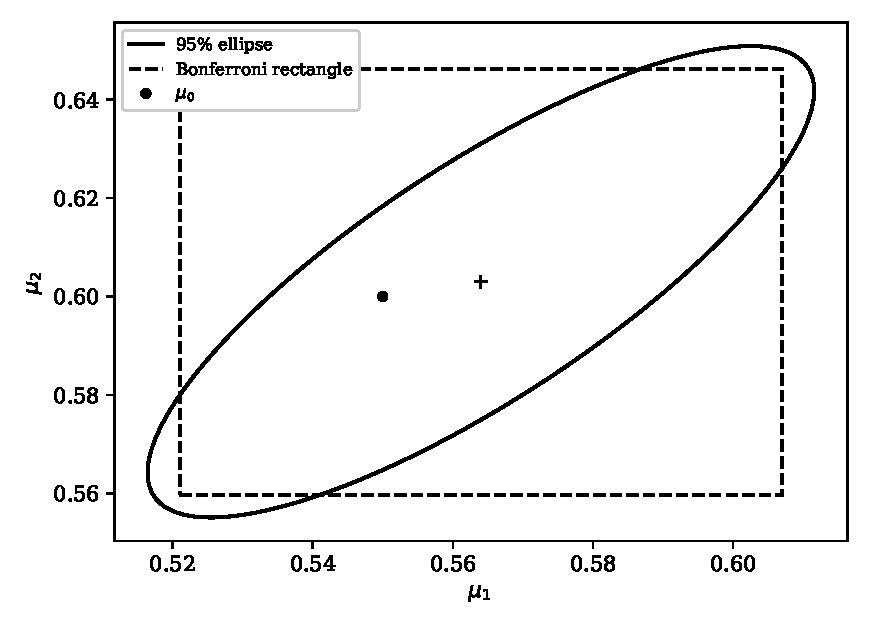
\includegraphics[width=.68\linewidth]{figures/5_5_ellipse.pdf}\end{center}
\textit{Độ chính xác dữ liệu:} Ví dụ 5.3 in $\mathbf S$ với bốn chữ số thập phân
nhưng in riêng $\mathbf S^{-1}$ với độ chính xác khác. Nghịch đảo của ma trận
$\mathbf S$ đã làm tròn không trùng hoàn toàn với ma trận nghịch đảo được in.
Ở đây dùng nhất quán $\mathbf S^{-1}$ đã cho; nếu nghịch đảo lại
$\begin{pmatrix}.0144&.0117\\.0117&.0146\end{pmatrix}$ thì $T^2=1.15000$,
quyết định không đổi. Hình vẽ dùng ma trận hiệp phương sai suy ra từ
$\mathbf S^{-1}$ để khớp với phép kiểm định.
\end{solution}

\begin{problem}[Bài 5.6.]
Chứng minh bất đẳng thức Bonferroni cho ba phát biểu.
\end{problem}
\begin{solution}
Gọi $C_i$ là biến cố phát biểu thứ $i$ đúng, $A_i=C_i^c$ là biến cố sai.
Với mọi kết quả của phép thử,
\[
\mathbf1_{A_1\cup A_2\cup A_3}\le
\mathbf1_{A_1}+\mathbf1_{A_2}+\mathbf1_{A_3}.
\]
Lấy kỳ vọng rồi dùng định luật De Morgan:
\[
\begin{aligned}
P(C_1\cap C_2\cap C_3)
&=1-P(A_1\cup A_2\cup A_3)\\
&\ge1-P(A_1)-P(A_2)-P(A_3)\\
&=P(C_1)+P(C_2)+P(C_3)-2.
\end{aligned}
\]
Nếu $P(C_i)\ge1-\alpha_i$, suy ra
\[
\answer{P(C_1\cap C_2\cap C_3)\ge1-(\alpha_1+\alpha_2+\alpha_3).}
\]
Đặc biệt, chọn $\alpha_i=\alpha/3$ bảo đảm xác suất cả ba phát biểu đúng
ít nhất $1-\alpha$. Chứng minh không cần các biến cố độc lập.
\end{solution}

\begin{problem}[Bài 5.7.]
Khoảng đồng thời cho ba trung bình của dữ liệu mồ hôi.
\end{problem}
\begin{solution}
Từ $20$ dòng trong Bảng 5.1, tính được
\[
\bar{\mathbf x}=(4.640,45.400,9.965)',\quad
\mathbf S=\begin{pmatrix}
2.879368&10.010000&-1.809053\\
10.010000&199.788421&-5.640000\\
-1.809053&-5.640000&3.627658
\end{pmatrix}.
\]
Với $p=3$, $\alpha=.05$, các hệ số là
\[
c_T=\frac{3(19)}{17}F_{3,17}(.95)=10.71860,\qquad
b=t_{19}(1-.05/6)=2.62511.
\]
Khoảng $T^2$ là $\bar x_j\pm\sqrt{c_Ts_{jj}/20}$,
còn Bonferroni là $\bar x_j\pm b\sqrt{s_{jj}/20}$.
\begin{center}\begin{tabular}{ccc}\toprule
Tham số & Khoảng $T^2$ & Khoảng Bonferroni\\\midrule
$\mu_1$ & $[3.3978,\;5.8822]$ & $[3.6440,\;5.6360]$\\
$\mu_2$ & $[35.0524,\;55.7476]$ & $[37.1031,\;53.6969]$\\
$\mu_3$ & $[8.5707,\;11.3593]$ & $[8.8470,\;11.0830]$\\
\bottomrule\end{tabular}\end{center}

Vì $\sqrt{c_T}=3.27393>b=2.62511$, các khoảng $T^2$ dài hơn khoảng
Bonferroni khoảng $24.7\%$ ở cả ba thành phần. Bonferroni phù hợp nếu chỉ
cần ba trung bình định trước; $T^2$ bảo đảm đồng thời cho mọi tổ hợp tuyến tính
$\mathbf a'\boldsymbol\mu$ nên có phạm vi suy luận rộng hơn.
\end{solution}

\begin{problem}[Bài 5.8.]
Hướng tổ hợp tuyến tính làm cực đại bình phương thống kê $t$.
\end{problem}
\begin{solution}
Với $\mathbf d=\bar{\mathbf x}-\boldsymbol\mu_0$, thống kê cho tổ hợp
$\mathbf a'\mathbf X$ là
\[
t^2(\mathbf a)=\frac{n(\mathbf a'\mathbf d)^2}{\mathbf a'\mathbf S\mathbf a}.
\]
Áp dụng Cauchy--Schwarz cho $\mathbf S^{1/2}\mathbf a$ và
$\mathbf S^{-1/2}\mathbf d$:
\[
(\mathbf a'\mathbf d)^2\le(\mathbf a'\mathbf S\mathbf a)
(\mathbf d'\mathbf S^{-1}\mathbf d).
\]
Dấu bằng đạt khi $\mathbf a=k\mathbf S^{-1}\mathbf d$, $k\ne0$, nên
$\max_{\mathbf a\ne0}t^2(\mathbf a)=T^2$.
Dùng dữ kiện Bài 5.5,
\[
\answer{\mathbf a=\begin{pmatrix}203.018&-163.391\\-163.391&200.228\end{pmatrix}
\begin{pmatrix}.014\\.003\end{pmatrix}
=\begin{pmatrix}2.352079\\-1.686790\end{pmatrix}.}
\]
Ta có $\mathbf a'\mathbf d=0.027868736$ và, vì $\mathbf S\mathbf a=\mathbf d$,
$\mathbf a'\mathbf S\mathbf a=0.027868736$. Do đó
\[
\answer{t^2(\mathbf a)=42\frac{(0.027868736)^2}{0.027868736}
=1.170486912=T^2.}
\]
Hướng này kết hợp cả hai biến; không thể chỉ nhìn hệ số lớn nhất để quy
kết toàn bộ khác biệt cho một biến, vì còn phụ thuộc đơn vị và tương quan.
\end{solution}

\begin{problem}[Bài 5.9.]
Suy luận đồng thời cho sáu kích thước cơ thể của gấu.
\end{problem}
\begin{solution}
Dữ kiện sách: $n=61$, $p=6$, $\bar{\mathbf x}=(95.52,164.38,55.69,93.39,17.98,31.13)'$,
\[
\mathbf S=\begin{pmatrix}
3266.46&1343.97&731.54&1175.50&162.68&238.37\\
1343.97&721.91&324.25&537.35&80.17&117.73\\
731.54&324.25&179.28&281.17&39.15&56.80\\
1175.50&537.35&281.17&474.98&63.73&94.85\\
162.68&80.17&39.15&63.73&9.95&13.88\\
238.37&117.73&56.80&94.85&13.88&21.26
\end{pmatrix}.
\]
Thứ tự biến: cân nặng, chiều dài cơ thể, vòng cổ, vòng ngực, chiều dài đầu,
chiều rộng đầu. Cân nặng tính bằng kg, các chiều dài tính bằng cm.
\textit{Lưu ý:} sách ghi $s_{66}=21.26$, khác $21.16$ trong ảnh đề Exercise 2.
\begin{enumerate}[label=\textbf{\alph*)}]
\item \textbf{Khoảng đồng thời mẫu lớn.}
Dùng $c_6=\chi_6^2(.95)=12.59159$:
\[
\answer{\mu_j\in\bar x_j\pm\sqrt{c_6s_{jj}/61},\quad j=1,\ldots,6.}
\]
Kết quả ở cột $T^2$ của bảng dưới được hiểu là \textit{xấp xỉ mẫu lớn}.
\item \textbf{Ellipse cho cân nặng và vòng ngực.}
Xét riêng $\boldsymbol\theta=(\mu_1,\mu_4)'$ với ma trận hiệp phương sai
\[
\mathbf S_{14}=\begin{pmatrix}3266.46&1175.50\\1175.50&474.98\end{pmatrix}.
\]
Với $u=\mu_1-95.52$, $v=\mu_4-93.39$,
\[
\answer{61(0.002798891u^2-0.013853621uv+0.019248107v^2)\le5.99146.}
\]
Vế phải là $\chi_2^2(.95)$ vì xét riêng cặp hai biến. Nếu chiếu miền sáu chiều
ở (a), vế phải phải giữ $\chi_6^2(.95)=12.59159$; đó là một ellipse lớn hơn.
\item \textbf{Bonferroni với $m=6$.}
Dùng $b_6=t_{60}(1-.05/12)=2.72855$:
\[
I_{B,j}=\bar x_j\pm b_6\sqrt{s_{jj}/61}.
\]
\begin{center}\begin{tabular}{ccc}\toprule
Tham số & Khoảng $T^2$ & Khoảng Bonferroni\\\midrule
$\mu_1$ & $[69.5535,\;121.4865]$ & $[75.5533,\;115.4867]$\\
$\mu_2$ & $[152.1728,\;176.5872]$ & $[154.9934,\;173.7666]$\\
$\mu_3$ & $[49.6067,\;61.7733]$ & $[51.0123,\;60.3677]$\\
$\mu_4$ & $[83.4882,\;103.2918]$ & $[85.7761,\;101.0039]$\\
$\mu_5$ & $[16.5469,\;19.4131]$ & $[16.8780,\;19.0820]$\\
$\mu_6$ & $[29.0351,\;33.2249]$ & $[29.5192,\;32.7408]$\\
\bottomrule\end{tabular}\end{center}

Các khoảng Bonferroni ngắn hơn vì $2.72855<\sqrt{12.59159}$.
Phân vị Student cho bảo đảm chính xác dưới giả thiết chuẩn; nếu chỉ dựa
vào mẫu lớn thì đây là xấp xỉ. Dùng thuần xấp xỉ chuẩn có thể thay hệ số
bởi $z(1-.05/12)=2.63826$.
\item \textbf{Hình chữ nhật Bonferroni.}
Giữ hiệu chỉnh $m=6$ theo đề:
\[
\answer{R_B=[75.5533,115.4867]\times[85.7761,101.0039].}
\]
Ellipse ở (b) nằm trong hình chữ nhật này vì hệ số nửa độ rộng chiếu
$\sqrt{\chi_2^2(.95)}=2.44775$ nhỏ hơn $b_6=2.72855$.
Ellipse phản ánh hiệp phương sai giữa hai biến; hình chữ nhật bảo đảm
cho cặp thành phần trong một họ gồm sáu phát biểu.
\begin{center}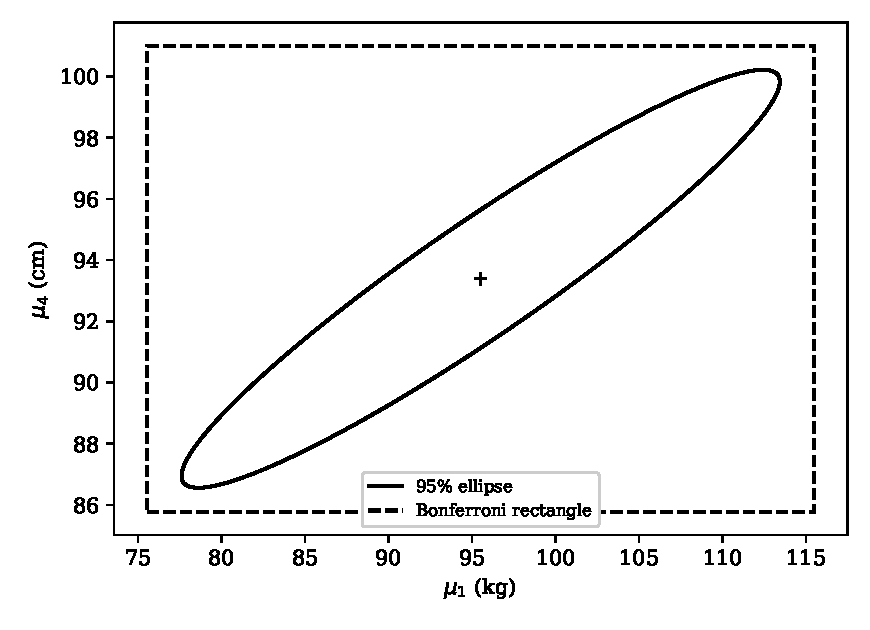
\includegraphics[width=.68\linewidth]{figures/5_9_ellipse.pdf}\end{center}
\item \textbf{Hiệu trung bình chiều rộng đầu trừ chiều dài đầu.}
Với $D=X_6-X_5$,
\[
\bar D=13.15,\qquad s_D^2=21.26+9.95-2(13.88)=3.45.
\]
Hiệu chỉnh cho $m=7$ đại lượng dùng $b_7=t_{60}(1-.05/14)=2.78547$, nên
\[
\answer{\mu_6-\mu_5\in13.15\pm2.78547\sqrt{3.45/61}
=[12.4876,13.8124]\ \text{cm}.}
\]
Nếu báo cáo cả bảy phát biểu như một họ đồng thời $95\%$, sáu khoảng ở (c)
cũng phải đổi sang hệ số $b_7$.
\end{enumerate}
\end{solution}

\begin{problem}[Bài 5.18.]
Dữ liệu điểm thi CLEP/CQT: kiểm định, trục ellipsoid và kiểm tra phân phối.
\end{problem}
\begin{solution}
Tính trực tiếp từ $87$ quan sát của Bảng 5.2:
\[
\bar{\mathbf x}=\begin{pmatrix}526.586207\\54.689655\\25.126437\end{pmatrix},\qquad
\mathbf S=\begin{pmatrix}
5808.059342&597.835204&222.029671\\
597.835204&126.053729&23.388532\\
222.029671&23.388532&23.111735
\end{pmatrix}.
\]
Tổng cột đầu là $45813$, do đó $\bar x_1=45813/87=526.586207$;
con số $526.29$ ở phần tóm tắt Ví dụ 5.5 không khớp bảng dữ liệu.
Lời giải này dùng bảng gốc, lưu kèm trong \texttt{data/college.csv}.
\begin{enumerate}[label=\textbf{\alph*)}]
\item \textbf{Kiểm định $H_0:\boldsymbol\mu=(500,50,30)'$.}
Với $\mathbf d=(26.586207,4.689655,-4.873563)'$,
\[
T^2=87\mathbf d'\mathbf S^{-1}\mathbf d=223.31018,
\quad c_T=\frac{3(86)}{84}F_{3,84}(.95)=8.33348.
\]
\[
\answer{F_{\mathrm{obs}}=72.70564,\quad\text{p-value}\approx2.83\times10^{-23};
\quad\text{bác bỏ }H_0.}
\]
Có bằng chứng rất mạnh rằng vectơ điểm trung bình của nhóm này khác
mức tham chiếu. Kết luận là về vectơ trung bình; để phát biểu riêng từng
thành phần có thể dùng các khoảng đồng thời sau:
\begin{center}\begin{tabular}{ccc}\toprule
Tham số & Khoảng $T^2$ & Khoảng Bonferroni\\\midrule
$\mu_1$ & $[502.9994,\;550.1730]$ & $[506.6359,\;546.5365]$\\
$\mu_2$ & $[51.2148,\;58.1645]$ & $[51.7506,\;57.6287]$\\
$\mu_3$ & $[23.6385,\;26.6143]$ & $[23.8679,\;26.3849]$\\
\bottomrule\end{tabular}\end{center}

Cả hai cách đều cho trung bình hai môn đầu cao hơn $500,50$, còn môn
khoa học thấp hơn $30$.
\item \textbf{Trục của ellipsoid $95\%$.}
Giải $\mathbf S\mathbf e_j=\lambda_j\mathbf e_j$ với $\|\mathbf e_j\|=1$.
Nếu $\boldsymbol\mu=\bar{\mathbf x}+\sum_jz_j\mathbf e_j$ thì phương trình miền là
\[
\sum_{j=1}^3\frac{z_j^2}{c_T\lambda_j/87}\le1.
\]
Nửa chiều dài trục là $h_j=\sqrt{c_T\lambda_j/87}$; chiều dài đầy đủ là $2h_j$.
\begin{center}
\begin{tabular}{cccc}
\toprule
$j$ & $\lambda_j$ & $h_j$ & $2h_j$\\\midrule
1 & 5878.791649 & 23.729998 & 47.459995\\
2 & 63.835100 & 2.472768 & 4.945537\\
3 & 14.598057 & 1.182500 & 2.365000\\\bottomrule
\end{tabular}
\end{center}
Các vectơ hướng tương ứng là
\[
\mathbf e_1=\begin{pmatrix}.993905\\.103443\\.038099\end{pmatrix},\quad
\mathbf e_2=\begin{pmatrix}-.103732\\.994589\\.005660\end{pmatrix},\quad
\mathbf e_3=\begin{pmatrix}-.037307\\-.009578\\.999258\end{pmatrix}.
\]
Hai đầu mỗi trục là $\answer{\bar{\mathbf x}\pm h_j\mathbf e_j}$.
Đổi dấu một vectơ riêng không thay đổi trục hình học.
\item \textbf{Q--Q plot và biểu đồ phân tán.}
\begin{center}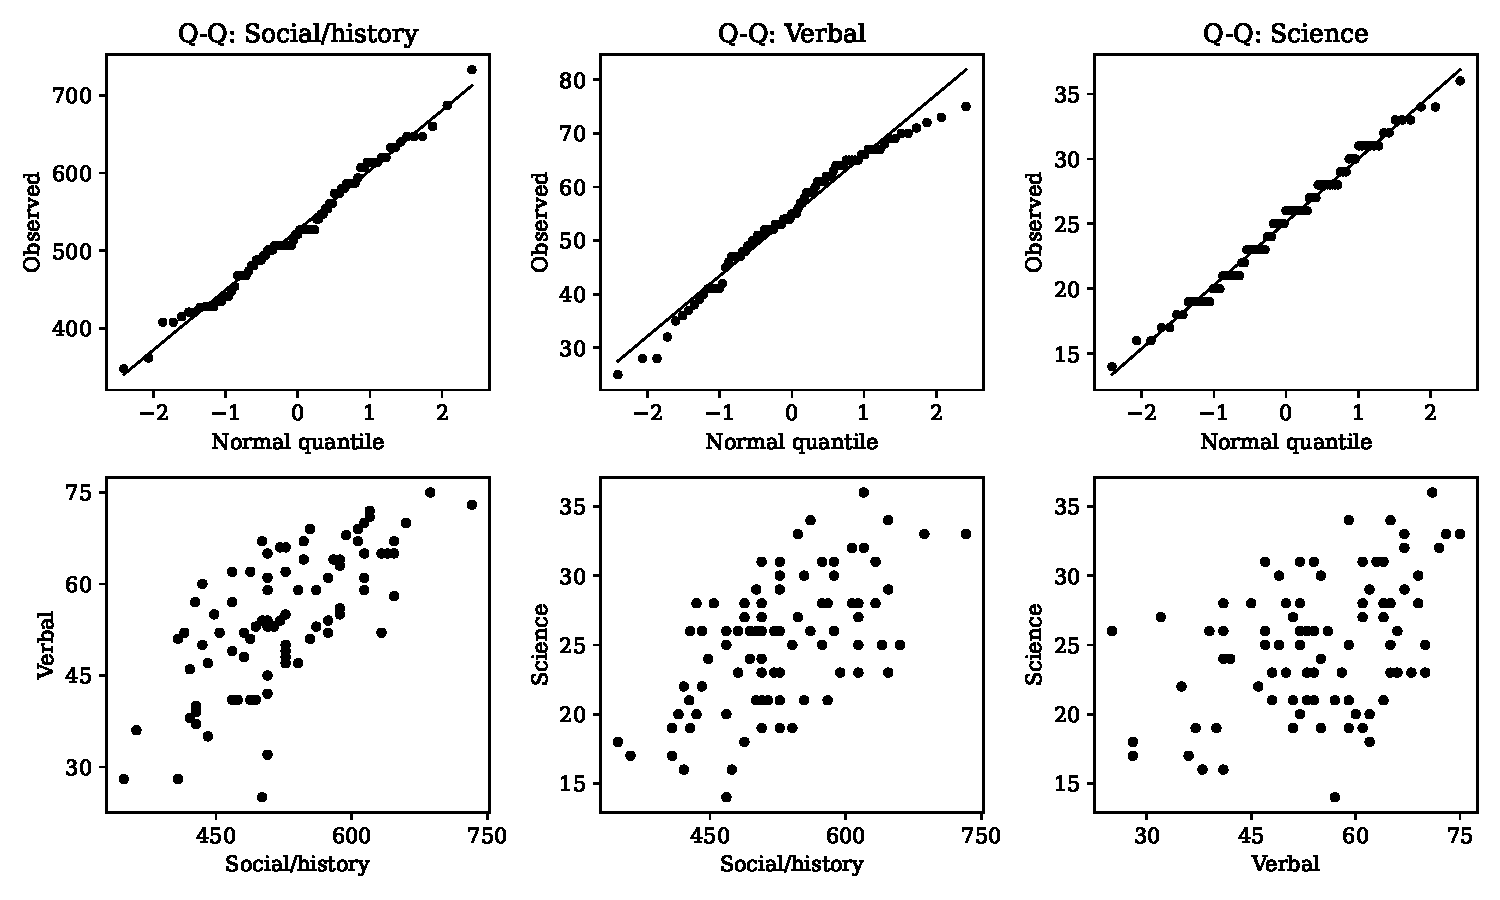
\includegraphics[width=\linewidth]{figures/5_18_diagnostics.pdf}\end{center}
Hai biến xã hội/lịch sử và khoa học bám khá sát đường chuẩn; biến ngôn ngữ
có lệch ở hai đuôi, nhất là các điểm thấp. Các đám mây điểm có xu hướng
liên hệ dương, không cho thấy tách nhóm rõ, nhưng giả thiết chuẩn ba chiều
chỉ nên xem là gần đúng. Kiểm tra phụ Shapiro--Wilk cho từng biên có
p-value lần lượt $0.6861,0.0387,0.5358$, củng cố việc thận trọng với biến ngôn ngữ.
Đây là các kiểm tra biên thăm dò, không phải kiểm định chuẩn nhiều chiều
và chưa hiệu chỉnh đa kiểm định. Với $n=87$, suy luận mẫu lớn cho vectơ
trung bình vẫn có cơ sở; chênh lệch kiểm định ở (a) rất lớn so với ngưỡng.
\end{enumerate}
\end{solution}

\begin{problem}[Bài 5.19.]
Dữ liệu gỗ: miền tin cậy hai chiều và tính phù hợp của giá trị tham chiếu.
\end{problem}
\begin{solution}
Từ $30$ cặp quan sát trong Bảng 5.11,
\[
\bar{\mathbf x}=(1860.5,8354.133333)',\qquad
\mathbf S=\begin{pmatrix}124054.672414&361620.448276\\
361620.448276&3486333.154023\end{pmatrix}.
\]
Các giá trị được giữ theo thang số của bảng; $X_1$ đo độ cứng và $X_2$
đo sức bền uốn.
\begin{enumerate}[label=\textbf{\alph*)}]
\item Đặt $\mathbf d_\mu=\boldsymbol\mu-\bar{\mathbf x}$. Miền cần vẽ là
\[
\answer{30\mathbf d_\mu'\mathbf S^{-1}\mathbf d_\mu\le
\frac{58}{28}F_{2,28}(.95)=6.91937.}
\]
Tâm ellipse là $\bar{\mathbf x}$ và các hướng trục là vectơ riêng của $\mathbf S$.
Nửa độ dài trục $j$ bằng $\sqrt{6.91937\lambda_j/30}$.
\begin{center}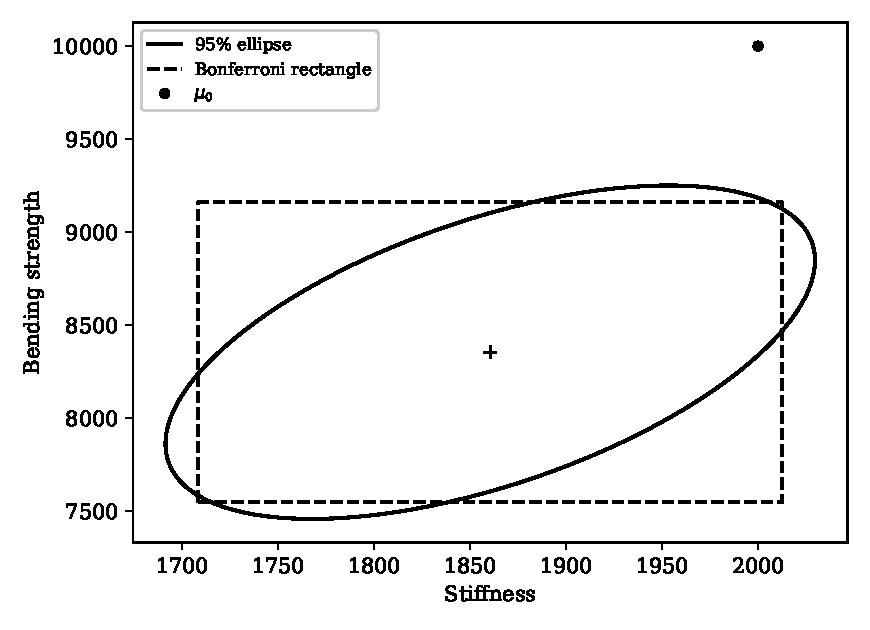
\includegraphics[width=.70\linewidth]{figures/5_19_ellipse.pdf}\end{center}
\item Với $\boldsymbol\mu_0=(2000,10000)'$, tính được
\[
T_0^2=23.64778>6.91937,\qquad
F_{\mathrm{obs}}=11.41617,\qquad\text{p-value}=0.0002367.
\]
\textbf{Điểm tham chiếu nằm ngoài ellipse}; dữ liệu không phù hợp với cặp
trung bình này ở mức $5\%$.
Để ôn thêm khoảng tin cậy thành phần như yêu cầu, ta có
\begin{center}\begin{tabular}{ccc}\toprule
Tham số & Khoảng $T^2$ & Khoảng Bonferroni\\\midrule
$\mu_1$ & $[1691.3472,\;2029.6528]$ & $[1708.4925,\;2012.5075]$\\
$\mu_2$ & $[7457.4128,\;9250.8538]$ & $[7548.3041,\;9159.9625]$\\
\bottomrule\end{tabular}\end{center}

\item Q--Q plot của hai biến gần tuyến tính, có dao động nhưng không cong
mạnh có hệ thống. Đám mây điểm có tương quan dương và không có tách nhóm
rõ; mô hình chuẩn hai chiều là một xấp xỉ khả dĩ. Các p-value Shapiro--Wilk
biên $0.6798$ và $0.6979$ không cho bằng chứng rõ chống lại tính chuẩn biên,
nhưng không chứng minh chuẩn đồng thời.
\begin{center}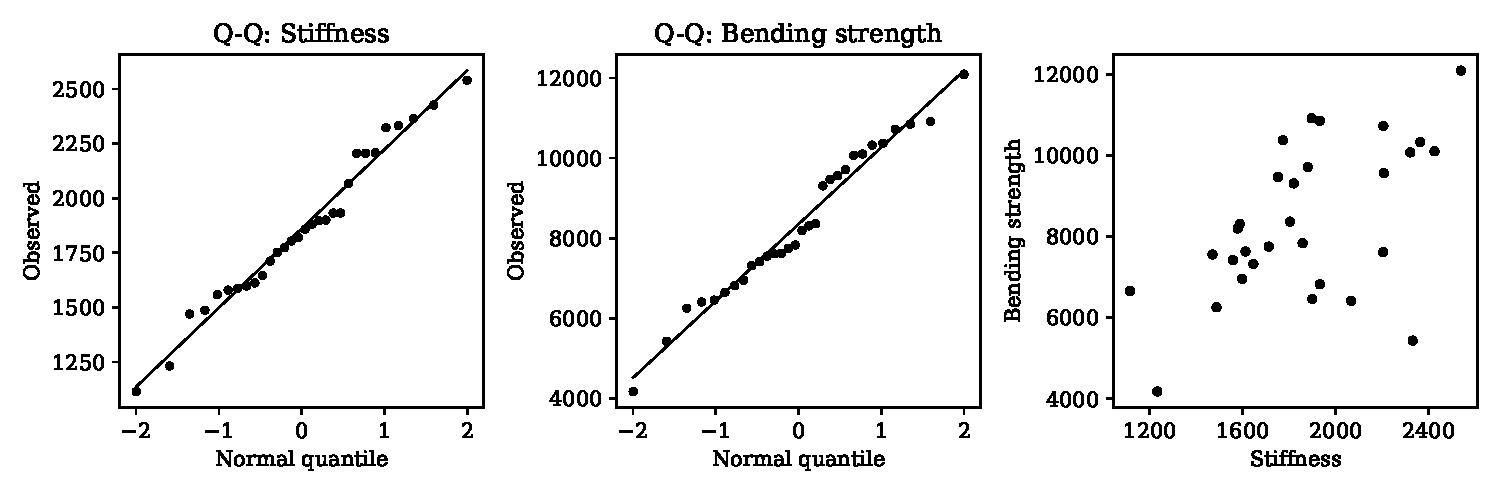
\includegraphics[width=.93\linewidth]{figures/5_19_diagnostics.pdf}\end{center}
\end{enumerate}
\end{solution}

\begin{problem}[Bài 5.20.]
Dữ liệu chim hook-billed kites: ellipse, khoảng đồng thời và kiểm tra phân phối.
\end{problem}
\begin{solution}
Bảng 5.12 gồm $45$ cặp chiều dài đuôi và cánh. Bản sách ghi $187$ và $268$
ở hai vị trí mà ảnh đề Exercise 2 ghi $287$ và $168$; vì thế kết quả dưới
đây được tính riêng theo dữ liệu sách, không sao chép kết quả Exercise 2.
\[
\bar{\mathbf x}=(193.622222,279.777778)',\qquad
\mathbf S=\begin{pmatrix}120.694949&122.345960\\122.345960&208.540404\end{pmatrix}.
\]
\begin{enumerate}[label=\textbf{\alph*)}]
\item Miền tin cậy $95\%$ là
\[
\answer{45(\boldsymbol\mu-\bar{\mathbf x})'\mathbf S^{-1}
(\boldsymbol\mu-\bar{\mathbf x})\le\frac{88}{43}F_{2,43}(.95)=6.57847.}
\]
Với cặp trung bình của chim đực $\boldsymbol\mu_0=(190,275)'$,
\[
T_0^2=5.54313<6.57847,\qquad\text{p-value}=0.07800.
\]
Cặp giá trị này nằm trong miền tin cậy nên vẫn hợp lý đối với trung bình
chim cái ở mức $5\%$; chưa đủ bằng chứng bác bỏ sự trùng nhau của hai giá trị
trung bình được xét. Đây không phải là khẳng định hai quần thể giống hệt nhau.
\begin{center}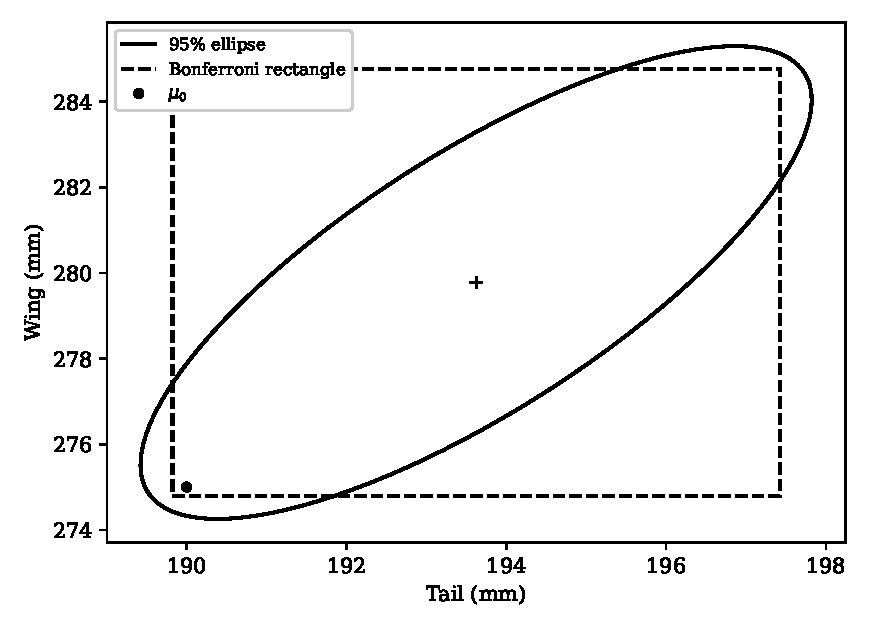
\includegraphics[width=.70\linewidth]{figures/5_20_ellipse.pdf}\end{center}
\item Các khoảng $T^2$ dùng hệ số $\sqrt{6.57847}=2.56485$.
Bonferroni cho hai trung bình dùng $t_{44}(.9875)=2.32071$:
\begin{center}\begin{tabular}{ccc}\toprule
Tham số & Khoảng $T^2$ & Khoảng Bonferroni\\\midrule
$\mu_1$ & $[189.4217,\;197.8227]$ & $[189.8216,\;197.4229]$\\
$\mu_2$ & $[274.2564,\;285.2992]$ & $[274.7819,\;284.7736]$\\
\bottomrule\end{tabular}\end{center}

Khoảng Bonferroni ngắn hơn. Khoảng $T^2$ có ưu điểm bảo đảm đồng thời cho
mọi tổ hợp tuyến tính, kể cả hướng lựa chọn sau khi xem dữ liệu, theo công thức
$\mathbf a'\bar{\mathbf x}\pm\sqrt{6.57847\mathbf a'\mathbf S\mathbf a/45}$.
Hiệu chỉnh Bonferroni $m=2$ ở trên chỉ bảo đảm cho hai trung bình định trước.
\item Hai Q--Q plot khá gần đường thẳng, biến đuôi có một số bậc do giá trị
lặp và sai lệch vừa phải ở đuôi. Biểu đồ phân tán có hướng tương quan dương,
không có điểm dị biệt cực đoan như sẽ xuất hiện nếu dùng $287$ hoặc $168$.
Mô hình chuẩn hai chiều là một xấp xỉ hợp lý cho bài tập, dù biểu đồ không
thể xác nhận chắc chắn chuẩn nhiều chiều. Kiểm tra biên Shapiro--Wilk cho
p-value $0.2857$ và $0.6726$.
\begin{center}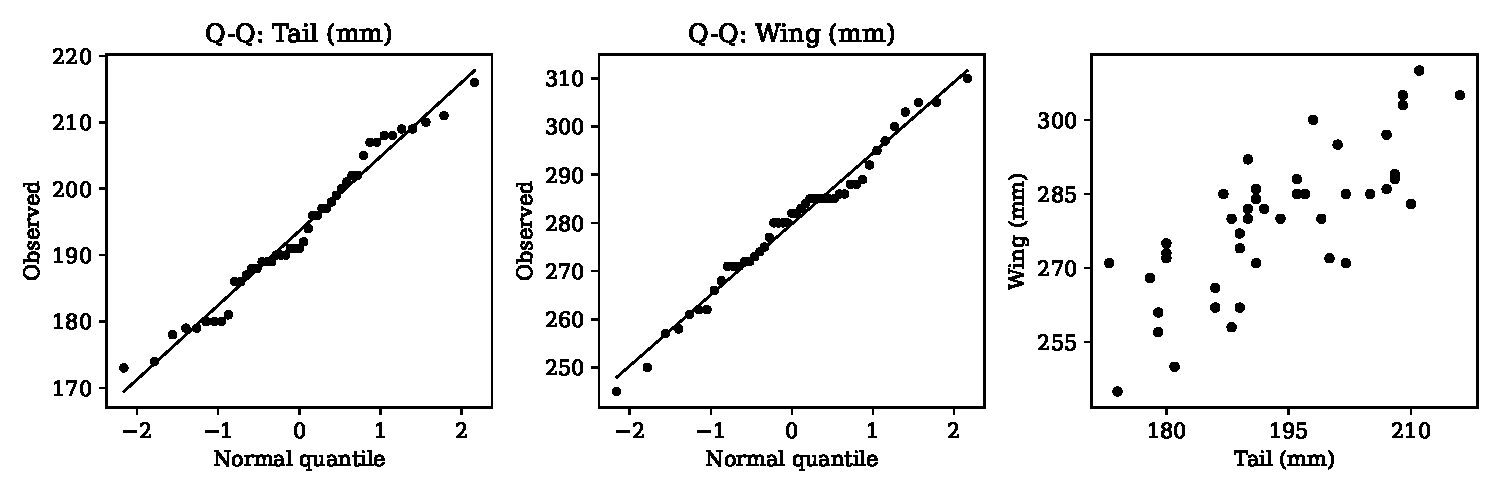
\includegraphics[width=.93\linewidth]{figures/5_20_diagnostics.pdf}\end{center}
\end{enumerate}
\end{solution}

\medskip
\noindent\textit{Nguồn đối chiếu đề và dữ liệu:} Johnson \& Wichern,
\textit{Applied Multivariate Statistical Analysis}, 6th ed., trang 200--205,
261--268; Bảng 5.1, 5.2, 5.11, 5.12 và Ví dụ 5.1, 5.3.
\href{https://www.stat.uchicago.edu/~lekheng/courses/331/books/Johnson-Wichern%20-%20Applied%20Multivariate%20Analysis.pdf}{Bản PDF trên website University of Chicago}.
Các file CSV, mã tính toán và hình vẽ đi kèm cho phép tái lập kết quả.
\vfill
\begin{center}{\small\itshape --- HẾT BÀI TẬP 3 ---}\end{center}
\end{document}
